\documentclass[12pt]{article}

\usepackage{amsmath, color}
\usepackage{mdwmath}
\usepackage{amssymb, epsf, epsfig, textcomp}
\renewcommand{\baselinestretch}{1.3}
\usepackage{a4wide}
\newcommand{\argmin}{\mathop{\mathrm{argmin}}}
\usepackage{caption}
\usepackage{subcaption}
\usepackage{mathtools}
\usepackage{listings}
\lstdefinestyle{myCustomMatlabStyle}{
	basicstyle=\ttfamily\tiny,
	breaklines=true,
	language=Matlab,
	numbers=left,
	stepnumber=1,
	numbersep=10pt,
	tabsize=4,
	showspaces=false,
	showstringspaces=false
}

\usepackage{sectsty}
\newcommand{\en}{\selectlanguage{english}}	% Set language to english
\newcommand{\el}{\selectlanguage{greek}}	% Set language to greek
\newcommand{\latin}[1]{\en#1\el}			% English text in greek text environment
\newcommand{\code}[1]{\texttt{\latin{#1}}}	% In-line code snippet
\newcommand{\unit}[1]{\text{\latin{ #1}}}	% For upright font in math mode
\newcommand\numberthis{\addtocounter{equation}{1}\tag{\theequation}}

\sectionfont{\fontsize{12}{15}\selectfont}

\begin{document}
	\noindent\rule{\textwidth}{2pt}
	\begin{center}
		{\bf Technical University of Crete}\\
		{\bf School of Electrical and Computer Engineering} \\
		Course: {\bf Convex Optimization} \\
		Exercise 3 (50/1000) \\
		Report Delivery Date: 7 December 2021 \\
		Instructor: Athanasios P. Liavas \\
	\end{center}
	{\bf Student: }Alevrakis Dimitrios 2017030001\\
	\rule{\textwidth}{.5pt}
	\vskip .1cm
	\noindent
	
	\begin{enumerate}
		\item[1.]Compute the projection of ${\bf x_0}\in \mathbb{R}^n$ onto the set $B({\bf 0}, r) \coloneqq\{{\bf x}\in\mathbb{R}^n | ||{\bf x||_2}\leq r\} $.
		\begin{enumerate}
			\item[(a)]
			\begin{figure}[h!]
				\begin{center}
					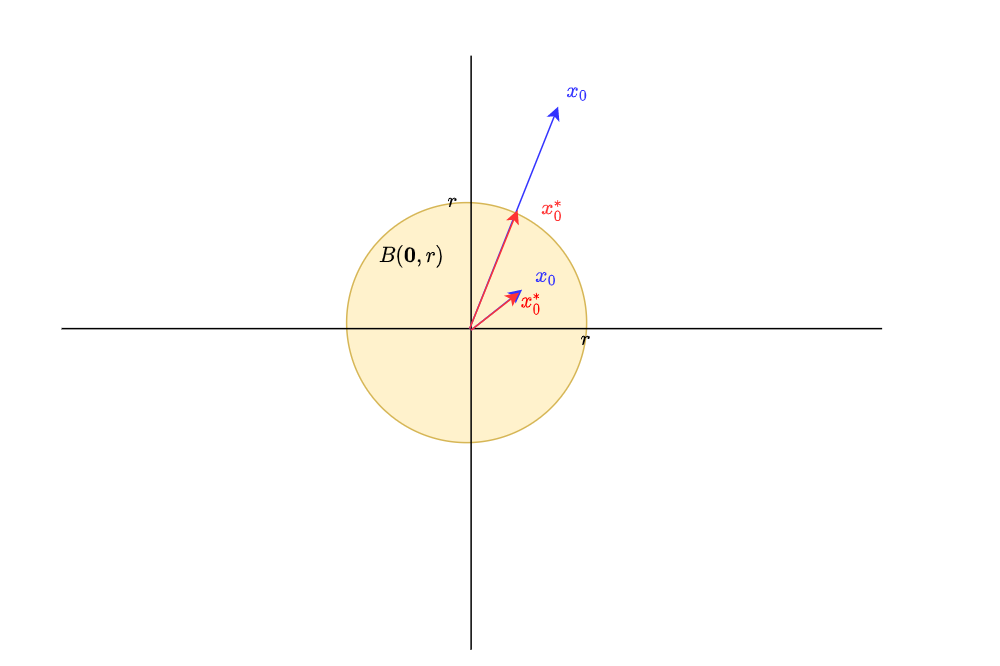
\includegraphics[width=1\linewidth]{1a}
				\end{center}
				\caption{Visualization of the problem in two dimensions. We discern the two possible cases for $x_0$ and its projections.}
			\end{figure}
			\item[(b)]
			We can discern two different cases for our problem.\\
			\begin{enumerate}
				\item[\bf Case 1]: 
				The vector ${\bf x_0}$ does not belong to the set $B({\bf 0},r)$ in which case we can see that the projection is the vector ${\bf x^*}\in B({\bf 0},r)$ for which is true that $||{\bf x^*}||_2=r$ and has the same angle as ${\bf x_0}$. The vector ${\bf x^*}$ can also be described as the vector ${\bf x^*}\in B({\bf 0},r)$ closer to ${\bf x_0}$.
				
				\item[\bf Case 2]:
				The vector ${\bf x_0}$ belongs to the set $B({\bf 0},r)$ in which case we can see that the projection of ${\bf x_0}$ is ${\bf x^*}={\bf x_0}$.
			\end{enumerate}
			We can therefore say for both cases that the computation of the projection can be written as:
			\begin{align*}
				&\text{minimize }f_0({\bf x})\coloneqq \frac{1}{2}||{\bf x_0}-{\bf x}||_2^2\\
				&\text{subject to }f_1({\bf x})=||{\bf x}||_2^2-r^2\leq 0 
			\end{align*}
			Instead of using $f_1(x)=||{\bf x}||_2-r\leq 0$ we can use  $f_1(x)=||{\bf x}||_2^2-r^2\leq 0$ for convenience since both $||x||_2$ and $r$ are non-negative.
			
			\item[(c)]
			The KKT equations:
			\begin{align*}
				&\nabla f_0({\bf x^*})+\lambda_*\nabla f_1({\bf x^*})=0 \numberthis \\
				&\lambda_*\geq0\\
				&f_1({\bf x^*})\leq 0\\
				&\lambda_*f_1({\bf x^*})=0
			\end{align*}
			Expanding (1):
			\begin{align*}
				&\nabla f_0({\bf x^*})+\lambda_*\nabla f_1({\bf x^*})=0 \iff\\
				&\nabla\big[\frac{1}{2}||{\bf x_0}-{\bf x^*}||_2^2\big]  +\lambda_*\nabla\big[||{\bf x^*}||_2^2-r^2\big]=0 \iff \\
				&{\bf x^*}-{\bf x_0}+2\lambda_*{\bf x^*}=0 \iff\\
				&(1+2\lambda_*){\bf x^*}-{\bf x_0}=0 \numberthis
			\end{align*}
		
			\item[(d)] 
			For $\lambda_*>0$:\\
			From the KKT equations: 
			\begin{align*}
				\lambda_*f_1({\bf x^*})=0 \overset{\lambda_*>0}{\iff}f_1({\bf x^*})=0 \iff ||{\bf x^*}||_2^2-r^2=0 \iff ||{\bf x^*}||_2^2=r^2 \iff ||{\bf x^*}||_2=r\numberthis
			\end{align*}
		
			Using (2):
			\begin{align*}
				&(1+2\lambda_*){\bf x^*}-{\bf x_0}=0 \iff {\bf x^*}=\frac{1}{1+2\lambda_*}{\bf x_0}\iff\\
				&||{\bf x^*}||_2=||\frac{1}{1+2\lambda_*}{\bf x_0}||_2 \overset{(3)}{\iff} r = \frac{1}{(1+2\lambda_*)}||{\bf x_0}||_2\iff\\
				&r+2r\lambda_*=||{\bf x_0}||_2 \iff \lambda_*=\frac{||{\bf x_0}||_2-r}{2r}>0
			\end{align*}
			
			Therefore ${\bf x^*}=r\frac{x_0}{||x_0||}$. Since for $\lambda_*>0$, $||{\bf x_0}|| > r$ we understand that ${\bf x_0}\notin B({\bf 0},r)$ and its projection is the vector normalized and scaled by a factor of $r$.\\
			
			\item[(e)]
			For $\lambda_*=0$: Using the equation (2): ${\bf x^*}={\bf x_0}$. From that we can conclude that ${\bf x_0}\in B({\bf 0},r)$ and therefore its projection onto $B({\bf 0},r)$ is itself.
			
			\item[Conclusion]:
			If ${\bf x_0}\in B({\bf 0},r)$ then ${\bf x^*}={\bf x_0}$ meaning the projection is ${\bf x_0}$ scaled by a factor of 1. In this case the fraction $\frac{r}{||x_0||_2}>1$. If ${\bf x_0}\notin B({\bf 0},r)$ then ${\bf x^*}=r\frac{x_0}{||x_0||}$ and $\frac{r}{||x_0||_2}<1$.\\
			Therefore for every case we can say that ${\bf x^*}=min\{1,\frac{r}{||x_0||_2}\}\cdot{\bf x_0}$
		\end{enumerate}
			
		\newpage
		\item[2.]
		Compute the projection of ${\bf x_0}\in \mathbb{R}^n$ onto the set $B({\bf y}, r) \coloneqq\{{\bf x}\in\mathbb{R}^n | ||{\bf x}-{}\bf y||_2\leq r\} $ for a given ${\bf y}\in\mathbb{R}^n$.
		
		\begin{enumerate}
			\item[(a)]
			\begin{figure}[h!]
				\begin{center}
					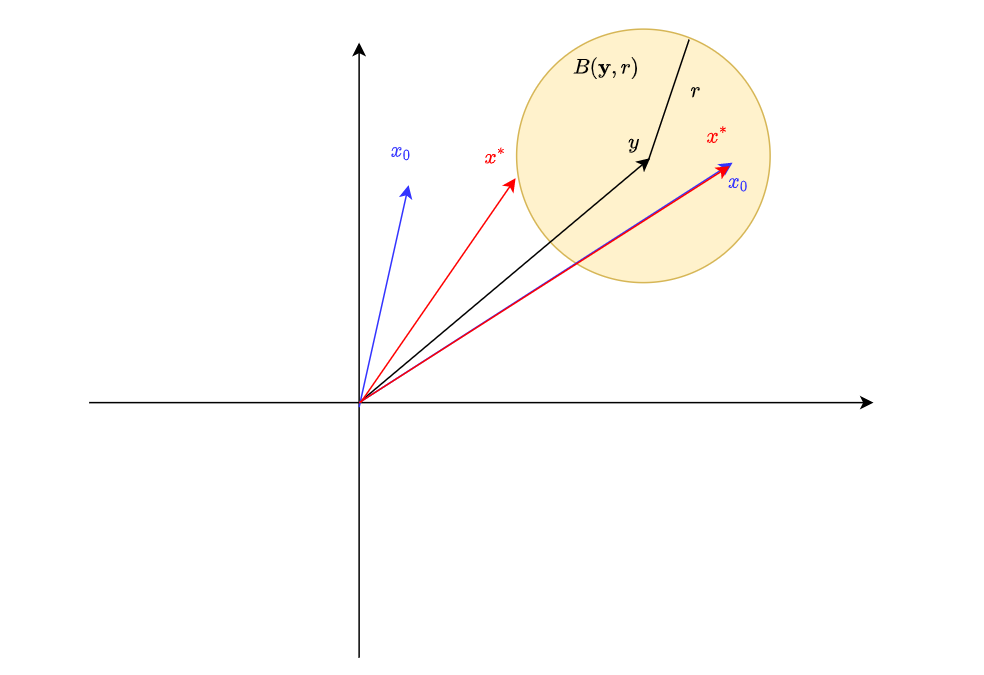
\includegraphics[width=1\linewidth]{2a}
				\end{center}
				\caption{Visualization of the problem in two dimensions. We discern the two possible cases for $x_0$ and its projections.}
			\end{figure}
			\item[(b)]
			Again the computation of the projection can be written as the problem:
			\begin{align*}
				&\text{minimize }f_0({\bf x})\coloneqq \frac{1}{2}||{\bf x_0}-{\bf x}||_2^2\\
				&\text{subject to }f_1({\bf x})=||{\bf x}-{\bf y}||_2^2-r^2\leq 0 
			\end{align*}
		
			\item[(c)]
			The KKT equations:
			\begin{align*}
				&\nabla f_0({\bf x^*})+\lambda_*\nabla f_1({\bf x^*})=0 \numberthis \\
				&\lambda_*\geq0\\
				&f_1({\bf x^*})\leq 0\\
				&\lambda_*f_1({\bf x^*})=0
			\end{align*}
		
			Expanding (4):
			\begin{align*}
				&\nabla f_0({\bf x^*})+\lambda_*\nabla f_1({\bf x^*})=0 \iff\\
				&\nabla\big[\frac{1}{2}||{\bf x_0}-{\bf x^*}||_2^2\big]  +\lambda_*\nabla\big[||{\bf x^*}-{\bf y}||_2^2-r^2\big]=0 \iff \\
				&{\bf x^*}-{\bf x_0}+2\lambda_*({\bf x^*}-{\bf y})=0 \iff\\
				&{\bf x^*}-{\bf y}+{\bf y}-{\bf x_0}+2\lambda_*({\bf x^*}-{\bf y})=0 \iff\\
				&(1+2\lambda_*)({\bf x^*}-{\bf y}) ={\bf x_0}-{\bf y}\numberthis
			\end{align*}
		
			\item[(d)] 
			For $\lambda_*>0$:\\
			From the KKT equations: 
			\begin{align*}
				&\lambda_*f_1({\bf x^*})=0 \overset{\lambda_*>0}{\iff}f_1({\bf x^*})=0 \iff ||{\bf x^*}-{\bf y}||_2^2-r^2=0 \iff \\
				&||{\bf x^*}-{\bf y}||_2^2=r^2 \iff ||{\bf x^*}-{\bf y}||_2=r\numberthis
			\end{align*}
			
			Using (5):
			\begin{align*}
				&(1+2\lambda_*)({\bf x^*}-{\bf y}) ={\bf x_0}-{\bf y}\iff\\
				&(1+2\lambda_*)||{\bf x^*}-{\bf y}||_2 = ||{\bf x_0}-{\bf y}||_2\overset{(6)}{\iff}\\
				&(1+2\lambda_*)r=||{\bf x_0}-{\bf y}||_2\iff\\
				&\lambda_*=\frac{||{\bf x_0}-{\bf y}||_2-r}{2r}>0
			\end{align*}
			
			Therefore since it must be true that $\lambda_*>0 \iff ||{\bf x_0}-{\bf y}||_2-r>0$ we understand that ${\bf x_0}\notin B({\bf y},r)$ and the projection:
			\begin{align*}
				(5)\Rightarrow {\bf x^*}&=\frac{{\bf x_0}-{\bf y}}{1+2\lambda_*}+{\bf y}=\frac{r}{||{\bf x_0}-{\bf y}||_2}(\bf {x_0}-{\bf y})+{\bf y}
			\end{align*}
		
			\item[(e)] 
			For $\lambda_*=0$: From (5) we get that ${\bf x^*}={\bf x_0}$ meaning that $x_0\in B({\bf y},r)$ and the projection of ${\bf x_0}$ on the set is itself.
		\end{enumerate}
		\newpage
		\item[3.]
		Let ${\bf a\in \mathbb{R}^n}$. Compute the projection of ${\bf x_0}$ onto set $\mathbb{S}\coloneqq\{{\bf x}\in \mathbb{R}^n | {\bf a\leq {\bf x}}\}$\\
		
		\begin{figure}[h!]
			\begin{center}
				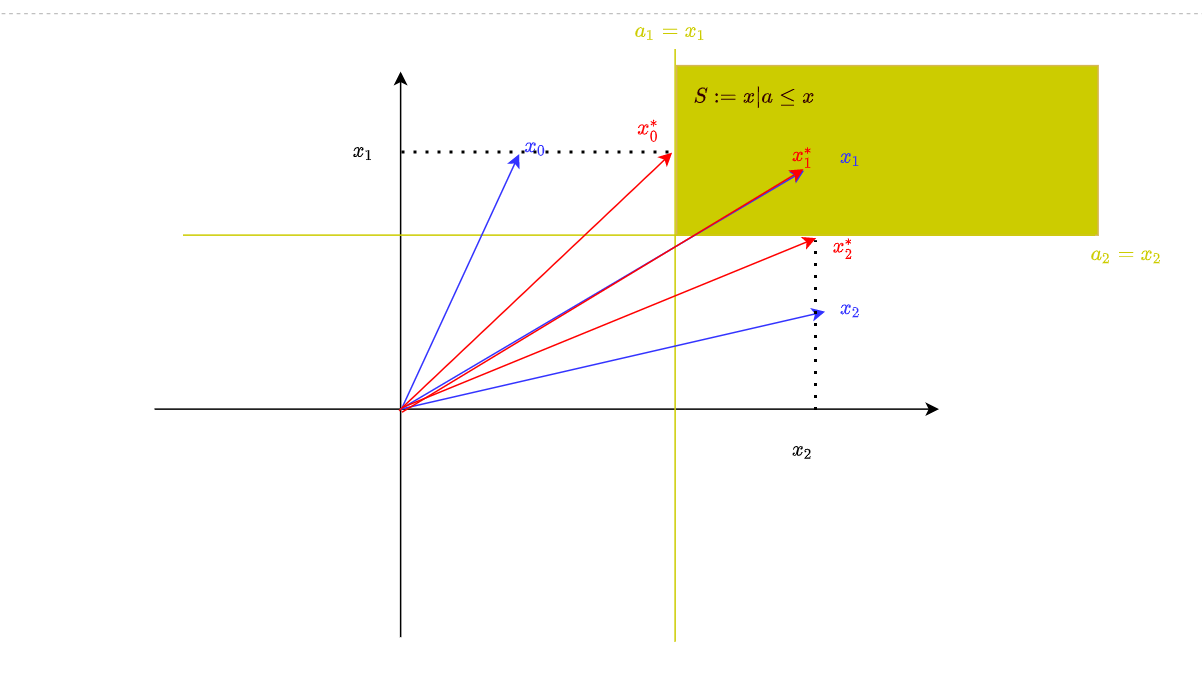
\includegraphics[width=1\linewidth]{3}
			\end{center}
			\caption{Visualization of the problem in two dimensions. We discern the three possible cases for $x_0$ and its projections.}
		\end{figure}
		The problem can be written as the minimization problem:
		\begin{align*}
			&\text{minimize }f_0({\bf x})\coloneqq \frac{1}{2}||{\bf x_0}-{\bf x}||_2^2\\
			&\text{subject to }f_i({\bf x})=a_i-x_i\leq 0,\ i=0,..,1
		\end{align*}
		
		The KKT equations:
		\begin{align*}
			\nabla f_0({\bf x^*})+\sum_{i=1}^{n}\lambda_i\nabla f_i({\bf x})&=0\numberthis\\
			\lambda_i&\geq0\, i=1,..,n\numberthis\\
			f_i({\bf x^*})&\leq 0,\ i=1,..,n\numberthis\\
			\lambda_if_i({\bf x^*})&=0,\ i=1,..,n\numberthis
		\end{align*}
		Defining ${\bf \lambda}\coloneqq(\lambda_1,..,\lambda_n)$ we can write equation (7) as:
		\begin{align}
			{\bf x^*}-{\bf x_0}-{\bf \lambda}=0 \Rightarrow {\bf x^*}={\bf x_0}+{\bf \lambda} \Rightarrow x^*_i = x_{0,i}+\lambda_i,\ i=1,..,n
		\end{align}
	
		We discern two cases:
		\begin{itemize}
			\item
			if $x_{0,1}< a_i:$
			\begin{align*}
				&x_{0,1}< a_i\Rightarrow x_{0,1}+\lambda_i< a_i+\lambda_i \overset{(11)}{\Rightarrow} x^*_i < a_i+\lambda_i \overset{(9)}{\Rightarrow}a_i\leq x_i^* < a_i +\lambda_i\\
				\\
				&\Rightarrow a_i< a_i +\lambda_i \Rightarrow \lambda_i > 0 \numberthis
			\end{align*}
			Therefore from (10) it must be true that $f_i({\bf x^*})=0 \Rightarrow a_i-x_i=0 \Rightarrow x_i = a_i$.
			
			\item
			if $x_{0,1}\geq a_i:$
			\begin{align*}
				&x_{0,1}\geq a_i\Rightarrow x_{0,1}+\lambda_i\geq a_i+\lambda_i \overset{(11)}{\Rightarrow} x^*_i \geq a_i+\lambda_i \overset{(9)}{\Rightarrow}a_i\leq x_i^* \geq a_i +\lambda_i\\
				\\
				&\overset{(8)}{\Rightarrow} \lambda_i = 0 \numberthis
			\end{align*}
			Therefore from (11): $x^*_i=x_{0,i}$.
		\end{itemize}
		Thus in general we can say that every element of the projection of ${\bf x_0}$ is given by $x^*_i=max\{a_i,x_{0,i}\},\ i,=1,..,n$
		\newpage
		\item[4.]
		Let ${\bf 0}\ne {\bf a}\in \mathbb{R}^n,\ b\in \mathbb{R}$. Solve the problem
		\begin{figure}[h!]
			\begin{center}
				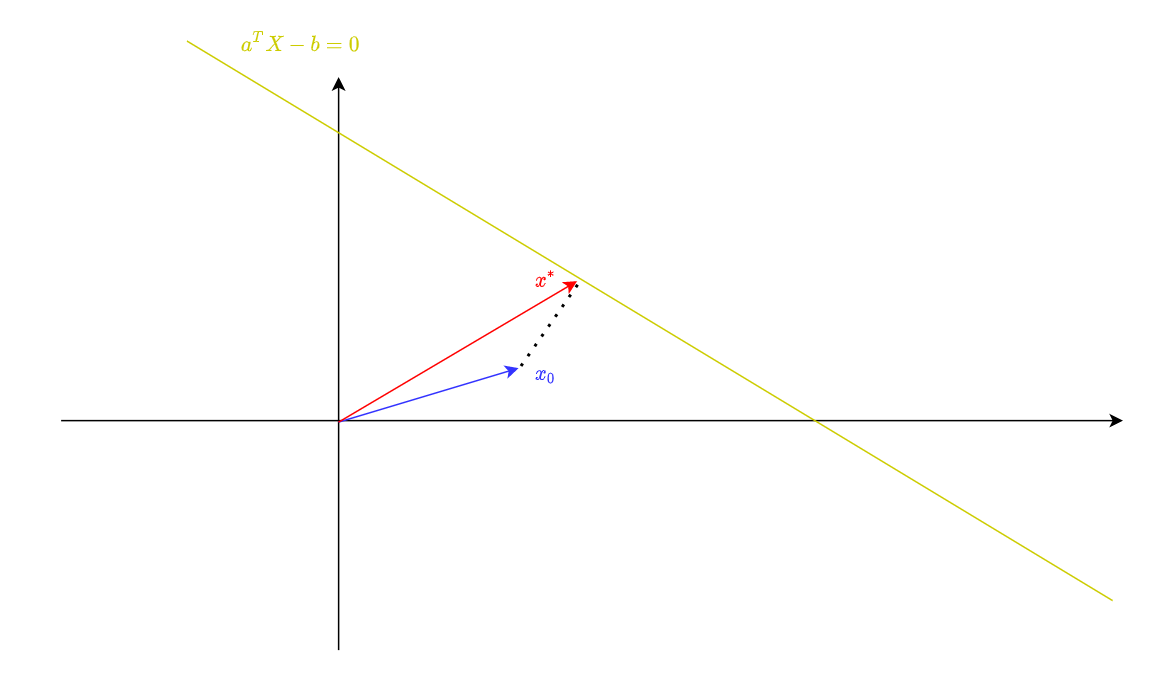
\includegraphics[width=1\linewidth]{4}
			\end{center}
			\caption{Visualization of the problem in two dimensions.}
		\end{figure}
		\begin{align*}
			&\text{minimize }\frac{1}{2}||{\bf x}||_2\\
			&\text{subject to }{\bf a}^T{\bf x}=b
		\end{align*}
		This problem is the same as :
		\begin{align*}
			&\text{minimize }f_0({\bf x})=\frac{1}{2}||{\bf x}||^2_2\\
			&\text{subject to }f_1({\bf x})={\bf a}^T{\bf x}-b=0 
		\end{align*}
		
		The KKT equations:
		\begin{align*}
			&\nabla f_0({\bf x^*})+u\nabla f_1({\bf x^*}) = 0,u\in\mathbb{R}\numberthis\\
			&f_1({\bf x^*})=0 \numberthis
		\end{align*}
		 
		Expanding(14):
		\begin{align*}
			(14)\Rightarrow {\bf x^*}+u{\bf a}=0 \Rightarrow {\bf x^*}=-u{\bf a}\numberthis
		\end{align*}
		
		Using (16) to (15):
		\begin{align*}
			f_1({\bf x^*})=0 \iff {\bf a}^T{\bf x}-b=0 	\iff{\bf a}^T(-u{\bf a}) -b= 0 \overset{{\bf a}{\iff}\ne{\bf 0}} u=-\frac{b}{||a||^2_2}\numberthis
		\end{align*}
	
		Therefore from (16) using (17): $\displaystyle{\bf x^*}=\frac{b}{||{\bf a}||_2^2}{\bf a}$
		
		\item[5.]
		Let {\bf A} $\mathbb{R}^{pxn}$, with $rank({\bf A})=p$, and ${\bf b}\in \mathbb{R}^p$. Find the distance from a point ${\bf x_0}\in \mathbb{R}^n$ from the set $\mathbb{S}\coloneqq\{{\bf x}\in \mathbb{R}^n|{\bf A}{\bf x}={\bf b}\}$.\\
		\begin{figure}[h!]
			\centering
			\begin{subfigure}[b]{0.45\textwidth}
				\centering
				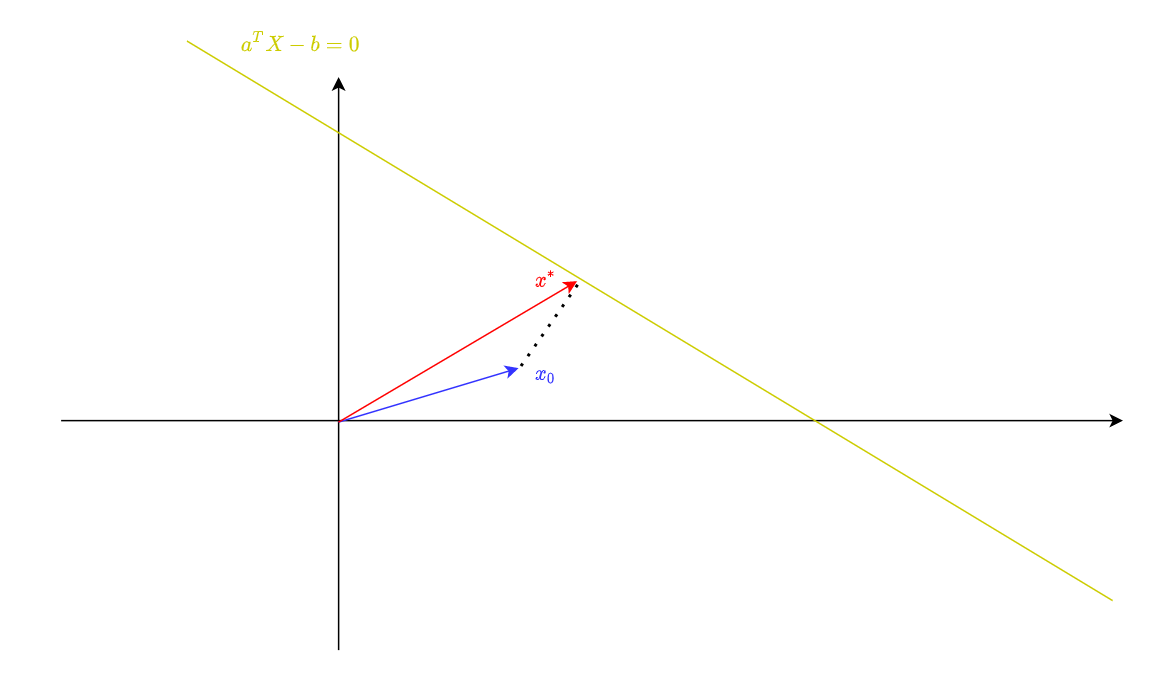
\includegraphics[width=\textwidth]{4.png}
				\caption{$p=1$}
			\end{subfigure}
			\hfill
			\begin{subfigure}[b]{0.45\textwidth}
				\centering
				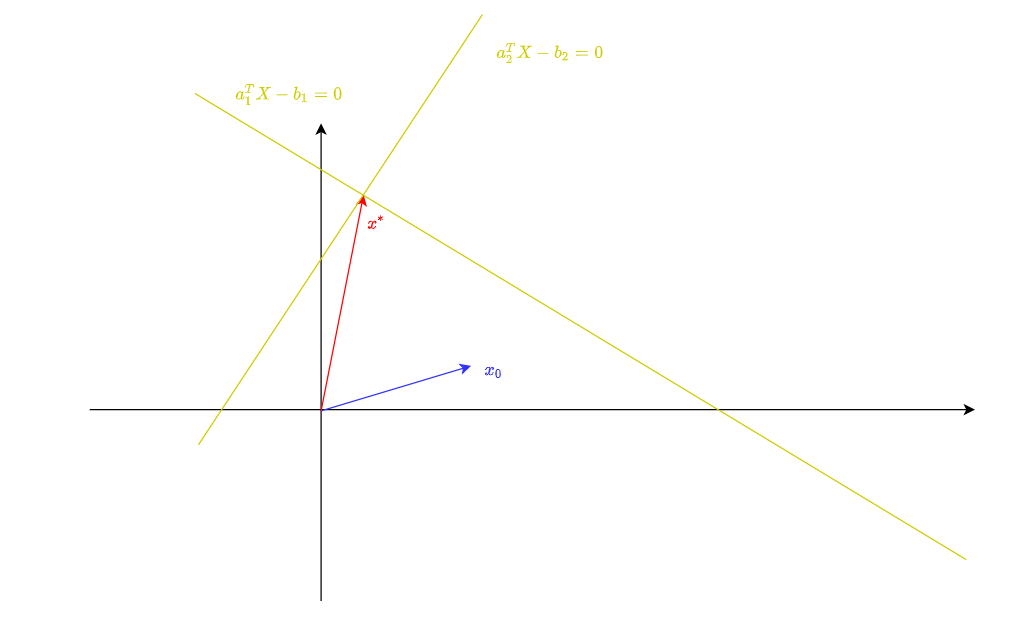
\includegraphics[width=\textwidth]{5a.png}
				\caption{$p=2$}
			\end{subfigure}
			\caption{Visualization of the problem for $n=2$. And since $n=2$, $p\leq 2$ to ensure row linear independence.}
		\end{figure}\\
		The problem:
		\begin{align*}
			\text{minimize }f_0({\bf x})=\frac{1}{2}||{\bf x}-{\bf x_0}||_2^2\\
			\text{subject to }f_1({\bf x}) = {\bf A}{\bf x}={\bf b}
		\end{align*}
	
		The KKT equations:
		\begin{align*}
			&\nabla f_0({\bf x^*})+{\bf A}^T{\bf v} = 0,u\in\mathbb{R}\numberthis\\
			&{\bf A}{\bf x^*}={\bf b} \numberthis
		\end{align*}
	
		Expanding (18):
		\begin{align*}
			{\bf x^*}-{\bf x_0}+{\bf A}^T{\bf v}={\bf 0} \iff {\bf x^*}={\bf x_0}-{\bf A}^T{\bf v}\numberthis
		\end{align*}
		
		Since $rank({\bf A})=p$ then ${\bf A}{\bf A}^T\in \mathbb{R}^{pxp}$ with $rank({\bf A}{\bf A}^T)=p$ therefore  ${\bf A}{\bf A}^T$ is invertible.
		Using (20) on (19):
		\begin{align*}
			{\bf A}({\bf x_0}-{\bf A}^T{\bf v})={\bf b}\iff {\bf v}=({\bf A}{\bf A}^T)^{-1}({\bf A}{\bf x_0}-{\bf b})\numberthis
		\end{align*}
	
		Thus: Using (21) on (20) : $\displaystyle {\bf x^*}={\bf x_0}-{\bf A}^T({\bf A}{\bf A}^T)^{-1}({\bf A}{\bf x_0}-{\bf b})$.
		
		So the distance of ${\bf x_0}$ from $\mathbb{S}$ is: 
		\begin{align*}
			||{\bf x^*}-{\bf x_0}||_2 = ||{\bf x_0}-{\bf A}^T({\bf A}{\bf A}^T)^{-1}({\bf A}{\bf x_0}-{\bf b})-{\bf x_0}||_2=||{\bf A}^T({\bf A}{\bf A}^T)^{-1}({\bf A}{\bf x_0}-{\bf b})||_2
		\end{align*}
	
		
	\end{enumerate}
\end{document}
